\documentclass[fleqn,10pt]{wlscirep}
\usepackage[utf8]{inputenc}
\usepackage[T1]{fontenc}
\usepackage{listings}
\usepackage{algorithm2e}
\usepackage{subcaption}
\usepackage[labelformat=parens,labelsep=quad,skip=3pt]{caption}
\usepackage{graphicx}

\title{AGEAS: Automated Machine Learning based Genetic Regulatory Element Extraction System}

\author[1,2,*1,+]{Jack Yu}
% \author[1,2,*1]{Jack Yu}
\author[2,+]{Masayoshi Nakamoto}
\author[1,*2,+]{Jiawang Tao}

% \author[2,+]{Derek Author}
\affil[1]{Center for Health Research, Guangzhou Institutes of Biomedicine and Health, Chinese Academy of Sciences, Guangzhou 510530, China}
\affil[2]{Shenzhen Mozhou Technology Co., Ltd, Shenzhen, China}
% \affil[2]{Affiliation, department, city, postcode, country}
\affil[*1]{Correspondence: gyu17@alumni.jh.edu}
\affil[*2]{Correspondence: tao\_jiawang@gibh.ac.cn}

\affil[+]{these authors contributed equally to this work}
\keywords{Machine Learning, Gene Regulatory Network, RNA-Seq, Chip-Seq}

\begin{abstract}
  As rapid progress in sequencing technology since last decade, numerous mechanisms underlying cell functions and developmental processes have been revealed as complex regulations of gene expressions.
  While single-cell RNA sequencing (scRNA-Seq) made high-resolution transcriptomic view increasingly accessible, precise identification of gene regulatory network (GRN) describing cell states became achievable.
  However, extracting key regulatory elements, including gene regulatory pathways (GRPs), transcription factors (TFs), and downstream genes, accurately reflecting main functionality changes remain challenging.
  Herein, we describe AGEAS, an automated machine learning (AutoML) based genetic regulatory element extraction system that assesses importances of GRPs in differentiating sample classes, such as cell types and developmental stages.
  With several case studies in divergent research areas, we show that AGEAS can indeed extract informative regulatory elements and reconstruct networks referring phenotype or biological process of interest.
  Furthermore, wet lab experiment validations...
  Overall, AGEAS provides an ...

  \subsection*{Availabilityand implementation}
  The AGEAS code is available at \url{https://github.com/JackSSK/Ageas}.
\end{abstract}

\begin{document}
\flushbottom
\maketitle

\thispagestyle{empty}
% \noindent Please note: Abbreviations should be introduced at the first mention in the main text – no abbreviations lists. Suggested structure of main text (not enforced) is provided below.

\section*{Introduction}
  \label{introduction}
  TBD
  % If analoging regulon with the graph concept in discrete mathematics, one of the most common methods to analyze influence of a vertex, which is equivalent to a gene, is assessing correspond degree of the vertex.
  % Although the regulatory source and target of GRP can be determined by utilizing interaction database, such as \emph{GTRD}\cite{gkaa1057} which shows regulatory relationship of interactors, numerous computational prediction methods like \emph{GRNBoost2}\cite{grnboost2} and comprehensive interaction database, \emph{BioGRID}\cite{biogrid} for example, could not provide faithful indication on regulatory directions.
  % Consequently, based on choice of interaction database, the regulon reconstructed with AGEAS cannot be guaranteed to be a directed graph but an undirected graph.
  % Therefore, in this step, \emph{odysseia} primarily extracts genes with high regulatory degrees in the regulon, regardless of they act as source or target in GRPs.
  % To limit total amount of output key genes, the default setting of AGEAS reconstructs regulon for top 100 GRPs, and genes with regulatory degree higher than two in the regulon will be considered influential.
  % If regulatory directions can be clarifed, the regulatory sources capable of regulating multiple key genes and the regulatory targets influenced by multiple key genes can also be extracted according to GRN reconstruction guidance.
  %
  % In the circumstance of finding genes potentially inducing CS conversion, referred as \emph{Mogrify}\cite{mogrify_2016}, both CS deterministic genes and common regulators of these genes shall gain attention.
  % Herein, AGEAS analogized key genes extracted from top GRPs as CS deterministic genes and TFs capable of regulating more than 2 listed key genes as significant common regulator.
  %
  % Both non-convergence issue and feature lost issue reflect on one of the key problems for $AutoML$: "No single machine learning method performs best on all datasets".\cite{NIPS2015_11d0e628}
  % Even though this problem can be solved while viewing $AutoML$ as a $CASH$ problem \cite{thornton2013auto}, such approach may not be directly deployable in our scenario considering comprehensive CS deterministic GFs or GRPs could be hardly labeled out.
  % Hence, in contrast with directly automating key features finding process, we decide to partially automate CS classification process and export candidate components of joint algorithm to feature importance analysis.
  % Compared with applying a particular $ML$ model, $CASH$ solving process during automation have higher potential to utilize comprehensive key features instead limited set of them.
  % Furthermore, due to the network-based essence of AGEAS, some CS deterministic features failed to be detected after classification model analysis, if having close regulatory relationships with multiple confirmed GFs, can still be traced down during regulon-based analysis at post stage analysis.

\section*{Method}
  \label{method}
  The basic principle of AGEAS is to find key regulatory elements associated with phenotype of interest through analyzing how well-performing classification models distinguish GRNs of sample with the phenotype from GRNs of samples without.
  To reconstruct sufficient GRNs for each class, RNA-Seq based expression data is segmented into subsets while each one is analogized as a pseudo-sample having discrete expression data.
  The pseudo-sample GRNs (psGRNs) are reconstructed accordingly; thus, classification models can be trained, evaluated, and interpreted having GRPs as input factors.
  With heavily weighted GRPs and associated genes repeatedly obtained from interpretations of success sample class predictions, GRNs could be formed and inferred playing important role in differentiating the studying sample classes.
  The overall workflow can be summarized as Figure \ref{workflow}.
  By default setting, four seperate extractor units in workflow run parallelly after data preprocessing part, and all extracted regulatory elements are used to form GRNs later combined into one atlas.
  Following sections describe each step of AGEAS in more depth.
  % \begin{itemize}
  %   \item \hyperref[step1]{\textbf{\emph{Step 1}}}: Data preprocessing
  %   \item \hyperref[step2]{\textbf{\emph{Step 2}}}: Classification model selection.
  %   \item \hyperref[step3]{\textbf{\emph{Step 3}}}: Feature selection...
  %   \item \hyperref[step4]{\textbf{\emph{Step 4}}}: Top GRP extraction.
  %   \item \hyperref[step5]{\textbf{\emph{Step 5}}}: Key network reconstruction.
  % \end{itemize}
  \begin{figure}[ht]
  \centering
  % 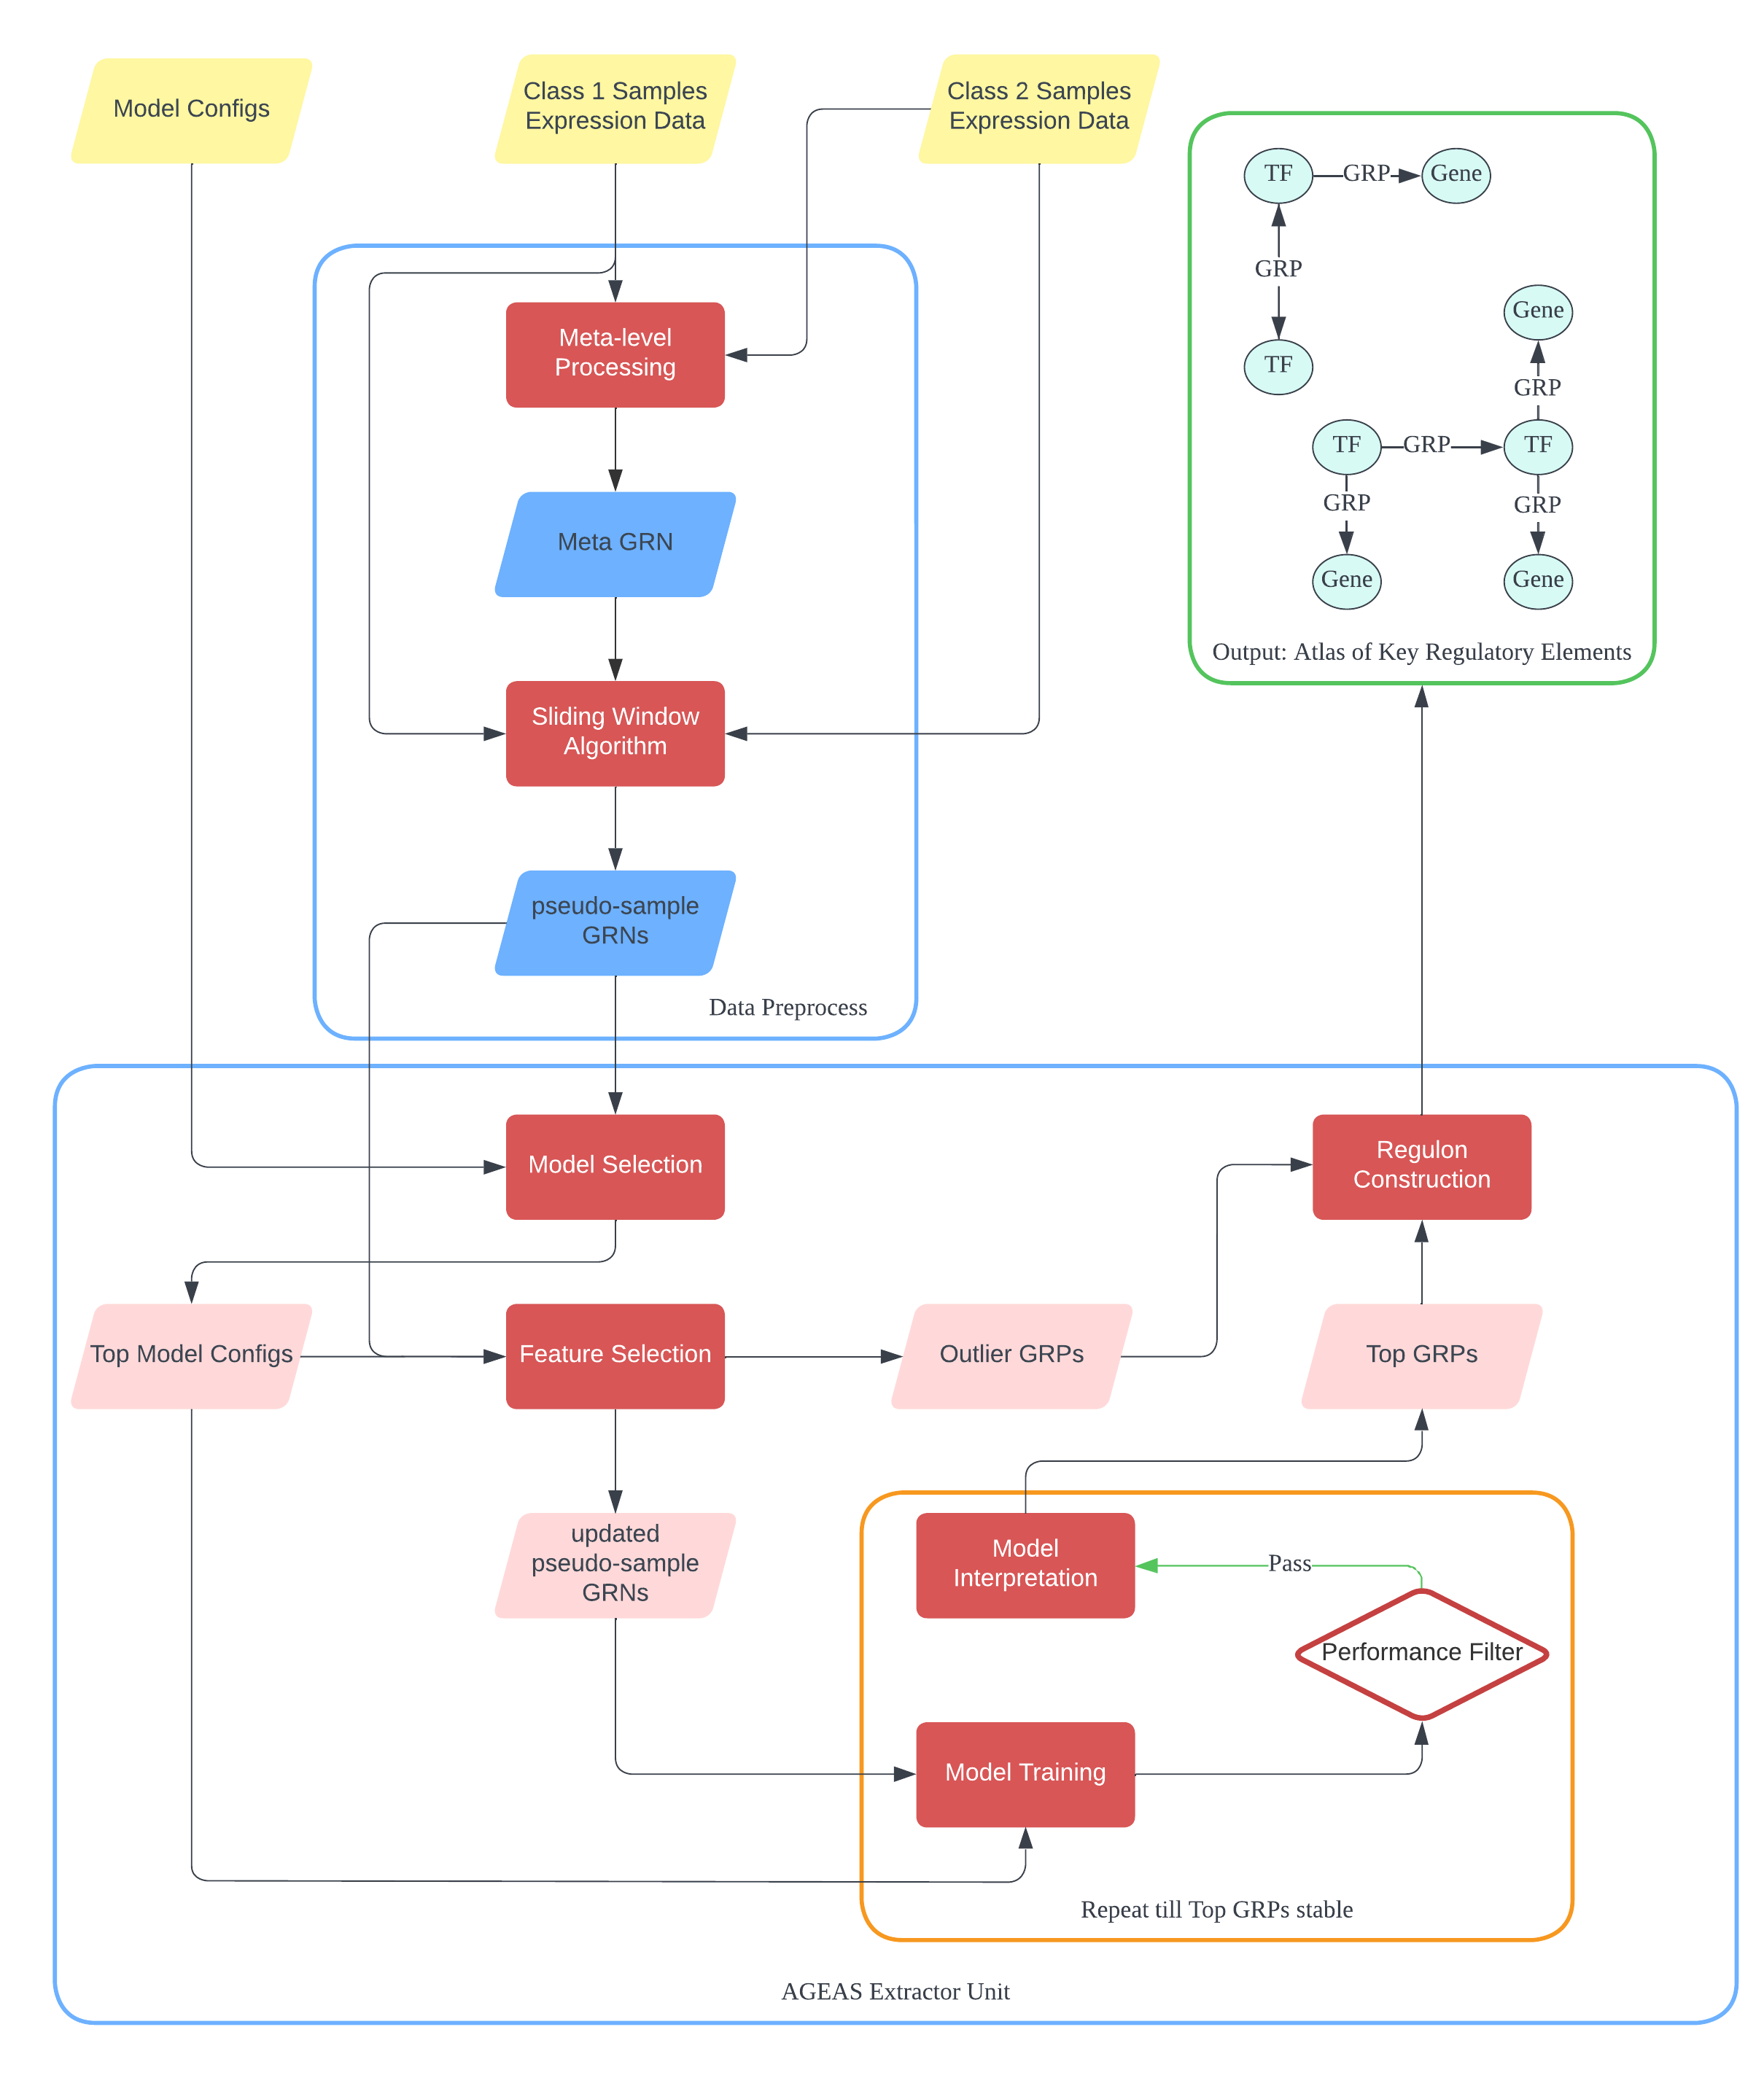
\includegraphics[width=0.8\linewidth, height=18cm, keepaspectratio,]{../images/summary_trans.png}
  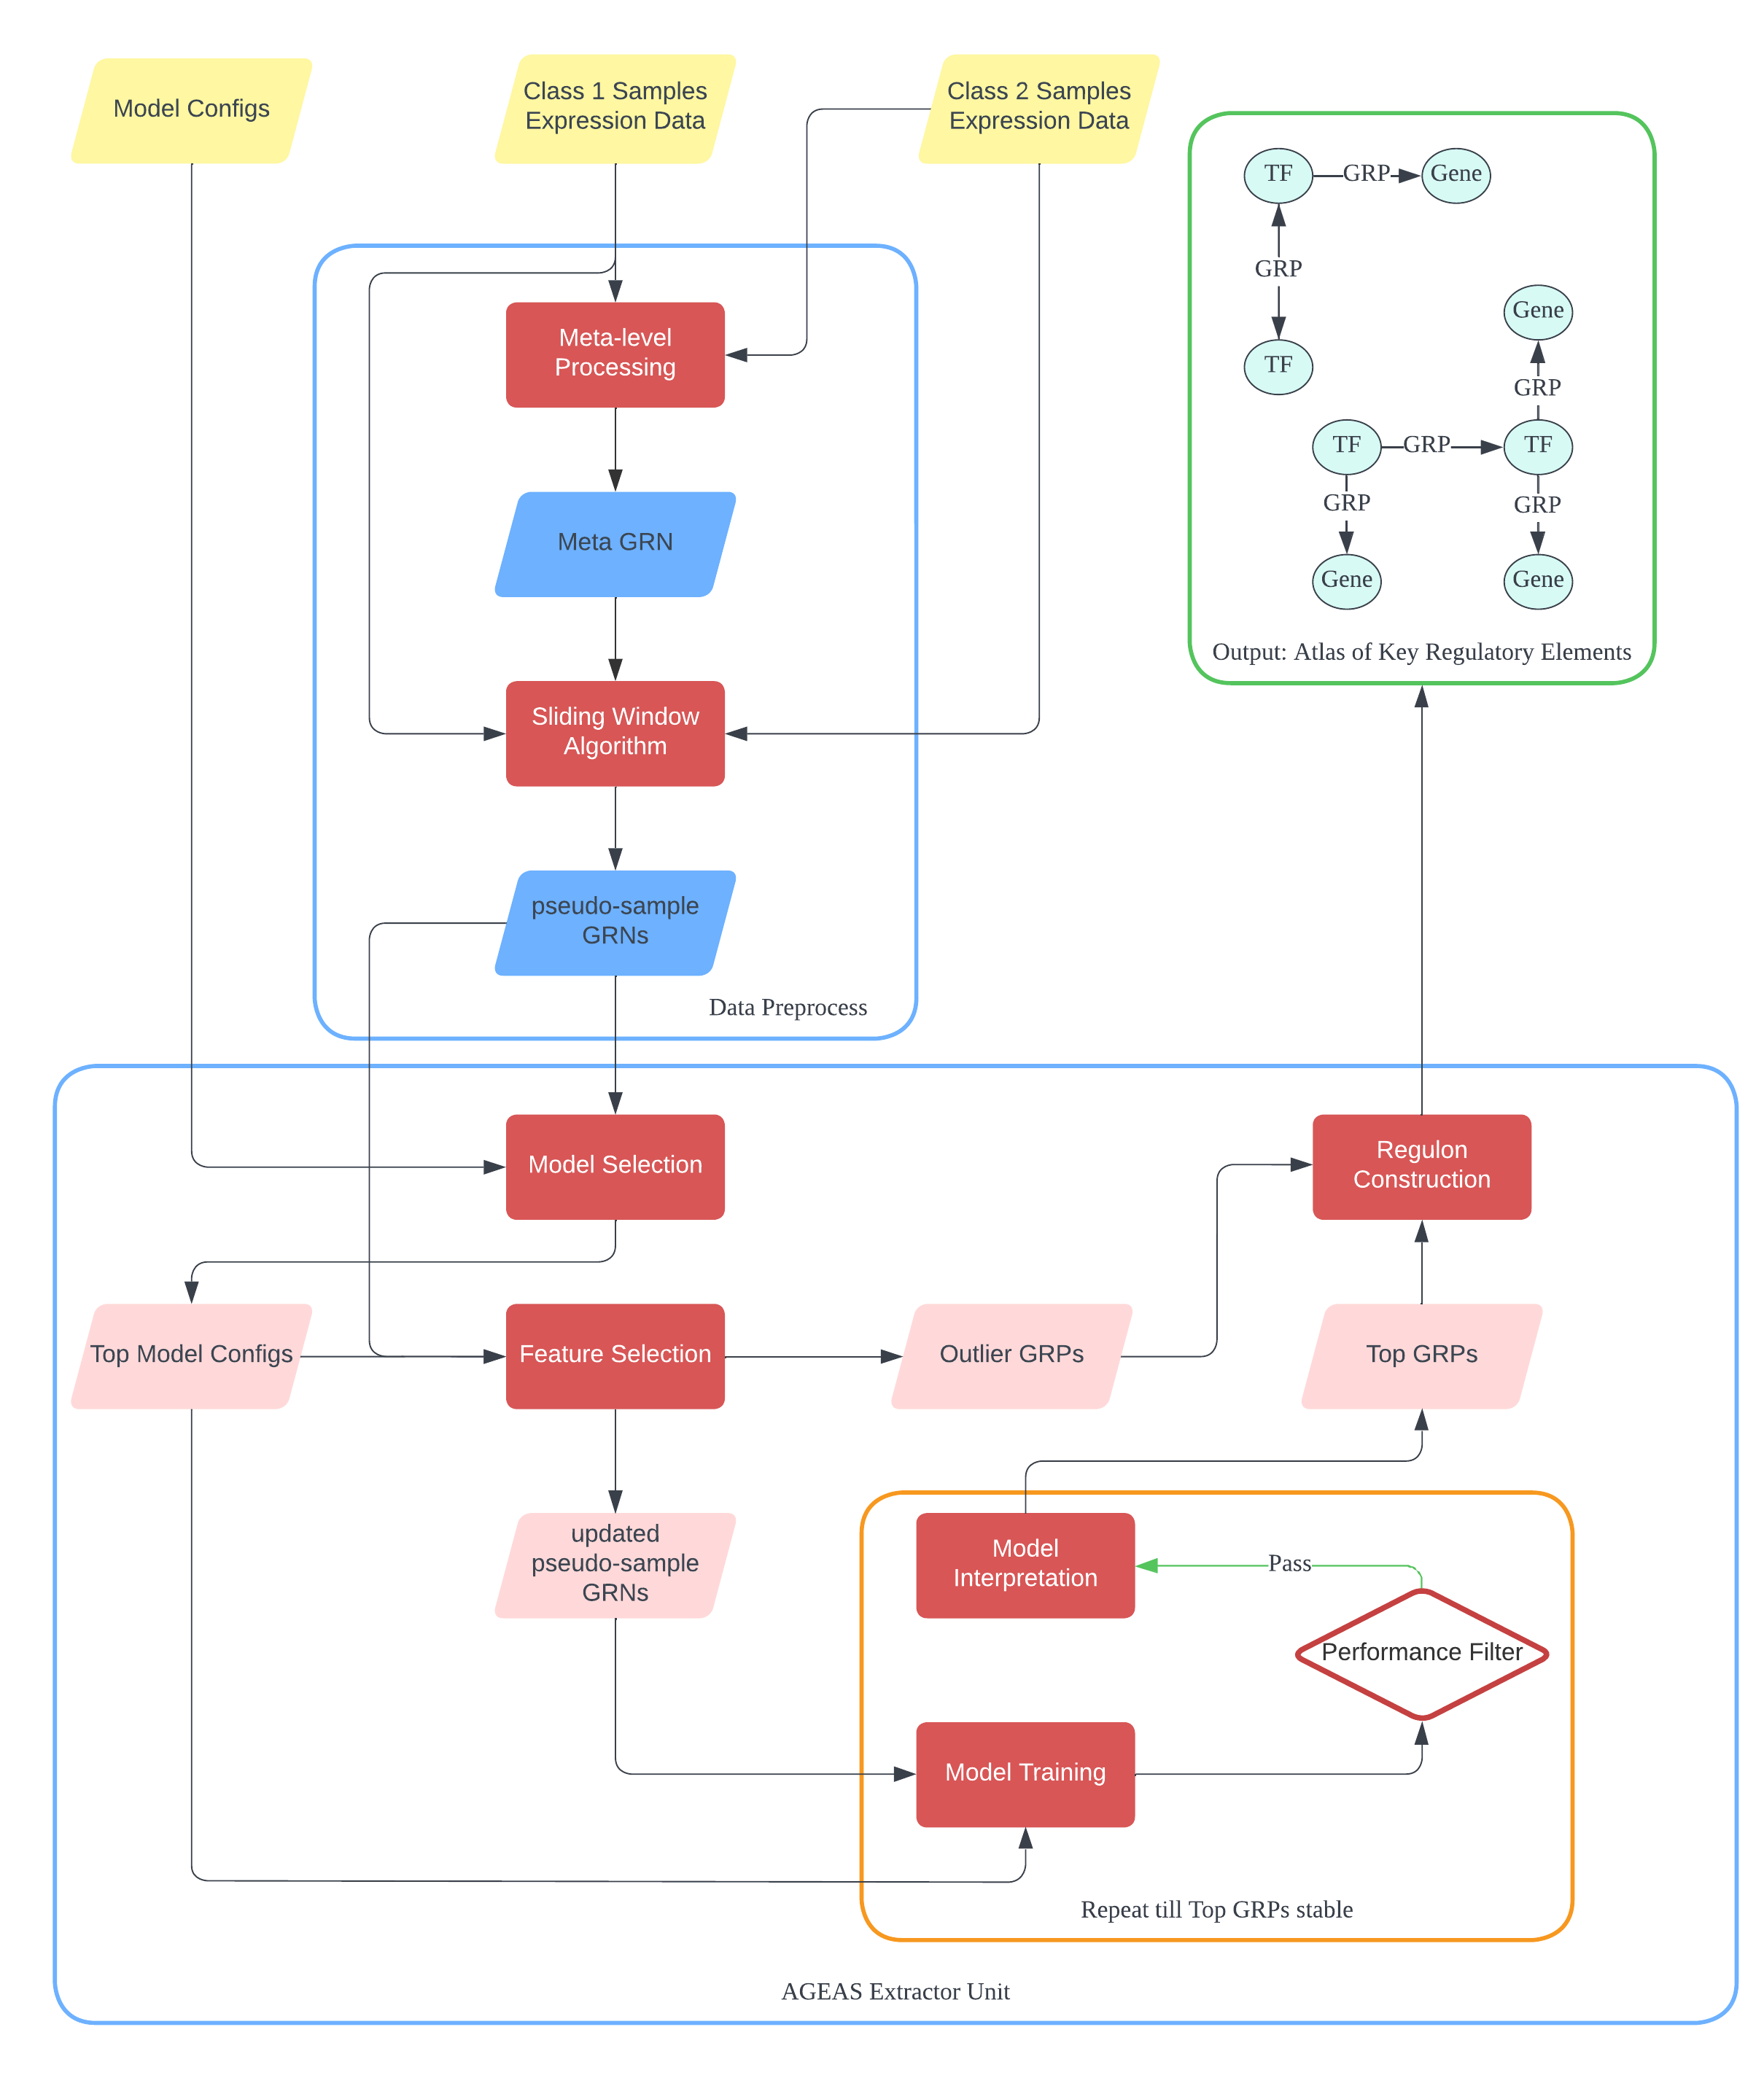
\includegraphics[width=0.8\linewidth, keepaspectratio,]{../images/summary_trans.png}
  \caption{
    The overall workflow of AGEAS:
    \textbf{\emph{(1)}} Reconstruct meta-level GRN (meta-GRN) with expression data of all samples.
    \textbf{\emph{(2)}} Build pseudo-samples with sliding window algorithm and reconstruct GRNs with GRPs identified in meta-GRN accordingly.
    \textbf{\emph{(3)}} Select best performing classifiers in predicting class labels of pseudo-sample GRNs (psGRNs).
    \textbf{\emph{(4)}} Interpret how top models make classifications and gradually exclude GRPs with low weights or outlier-level high weights.
    \textbf{\emph{(5)}} Repeatedly train classifiers with differnt set of psGRNs as training data to extract GRPs frequently ranked as top important features for decision.
    \textbf{\emph{(6)}} Reconstruct GRNs with extracted GRPs and GRPs excluded as significant outliers.
  }
  \label{workflow}
  \end{figure}

  \subsection*{Step 1:Data preprocessing}
    \label{step1}
    The main purpose of this step is to build pseudo-samples and reconstruct corresponding pseudo-sample GRNs (psGRNs).
    % Instead of finding genes being important to differentiate sample classes and infer gene regulatory networks (GRNs) with the genes,
    For each sample class, gene expression matrices (GEMs) labeled with same class label are concatenated as one comprehensive expression matrix.
    With comprehensive GEMs, a meta-level GRN (meta-GRN) is reconstructed in advance of psGRNs to provide generic guidance on reconstruction.
    In general, the workflow of this step can be represented as Figure \ref{data_preprocess}.

    \subsubsection*{Reconstruct meta-GRN}
      Firstly, genes included in the comprehensive GEMs are assessed and determined whether having potential to form informative GRPs with other genes.
      Commonly, differentially expressed genes (DEGs) would be considered as important factors of studying feature.
      Here we apply the Mann-Whitney U rank test (MWW) implemented by \emph{SciPy}\cite{2020SciPy-NMeth} to exclude genes having indistinguishable expression level distribution across GEMs of different classes.
      The p-value for rejecting null hypothesis, that expression distribution underlying class 1 samples is the same as the expression distribution underlying class 2 samples, is set to 0.05 by default.
      Furthermore, a $\log_2$ fold change (log2FC) filter is also implemented in AGEAS.
      However, enabling the log2FC filter is not encouraged considering upstream TFs indirectly regulating key genes associated with feature of interest may not always have significant expression level difference between sample classes.
      The lof2FC filter shall mostly be used in order to decrease meta-GRN's GRP total amount in a compromising position caused by limited computational resources.
      After differential expression based filters, a standard deviation ($\sigma$) filter is applied to exclude genes either having low expression value or merely affected by dynamic expression status of other genes.
      By default, the $\sigma$ threshold is set to 1.0, the lowest expression level in raw gene count matrix gained from RNA-Seq data.
      The threshold value should be adjusted corresponding to prior knowledge of input GEMs, for example of what normalization method was applied to the GEMs.

      With candidate genes passed filters above, some gene pairs are formed and assessed potential of representing GRPs.
      To reduce overall computational complexity, a gene pair shall be formed with at least one TF which could be the regulatory source of GRP.
      If not further specified, TF list will be retrieved from integrated \emph{TRANSFAC}\cite{transfac} datasets according to the provided species information.
      Utilizing genetic interaction database like \emph{GTRD}\cite{gkaa1057} and \emph{BioGRID}\cite{biogrid}, AGEAS checks whether the binding ability of gene pair is confirmed or not.
      By default, if TF being recorded to have binding site within target gene's promoter range (-1000 to +100) by Chromatin Immunoprecipitation Sequencing (ChIP-Seq) dataset retrieved from \emph{GTRD}\cite{gkaa1057}, the potential GRP gene pair will be passed to expression correlation assessment.
      For TFs not covered by interaction database, \emph{GRNBoost2}\cite{grnboost2}-like algorithm is initiated to predict potential regulatory target genes.
      The prediction importance threshold can either be set manually or automatically based on recorded interactions as:

      \centerline{$Threshold = min(GA(M_1, t)\, \uplus \, GA(M_2, t), \frac{1}{g})$}

      \noindent Here $GA()$ denotes \emph{GRNBoost2}\cite{grnboost2}-like algorithm;
      $M_1$ is concatenated class 1 samples GEM with genes passed filters;
      $M_2$ is concatenated class 2 samples GEM with genes passed filters;
      $t$ is the TF having largest amount of recorded interaction in dataset;
      $g$ is total amount of unique genes in all samples passed filters.

      After potential GRP gene pairs obtained, a expression correlation filter is used to exclude gene pairs having low covariance which implies weak relationship.
      To assess expression correlation, AGEAS applies Pearson's Correlation coefficient\cite{pcc_2012} (PCC) whihc is one of the widely adopted methods.\cite{cid_2019}
      With default setting, gene pairs can reach absolute correlation coefficient of 0.2 while keeping correspond p-value lower than 0.05 are included in meta-GRN as validated GRP.

    \subsubsection*{Reconstruct psGRNs}
      The comprehensive GEMs is divided into few sample subsets with sliding window algorithm (SWA) to build pseudo-samples.
      With SWA, we can gain GEM of \emph{i-th} pseudo-sample through:

      \centerline{$SWA(i) = \left\{{x_j}_{j = i * p}^{j + k}\right\}, j + k < l$}

      \noindent Here $l$ is number of samples in a comprehensive GEM which can be expressed as $\left\{{x_j}_{j = 0}^{l}\right\}$; $k$ denotes window size; $p$ denotes padding stride.

      If sample amount is considerably low or imbalanced, customized window size and padding stride can be applied to generate sufficient amount of pseudo-samples for later classifier training and assessment processes.
      Utilizing meta-GRN, psGRNs are reconstructed with GEMs of pseudo-sample.
      Each GRP gene pair in meta-GRN is formed with expression data in pseudo-sample and filtered by same PCC filter in meta-GRN reconstruction process.

      After all pseudo-samples have been used to reconstruct psGRN, every psGRN can be represented as matrix comprising GRPs' PCC values.
      The order of GRPs in each psGRN is also unified through adding GRPs included in other psGRNs with 0.0 PCC value.

    \begin{figure}[ht]
      \centering
      % 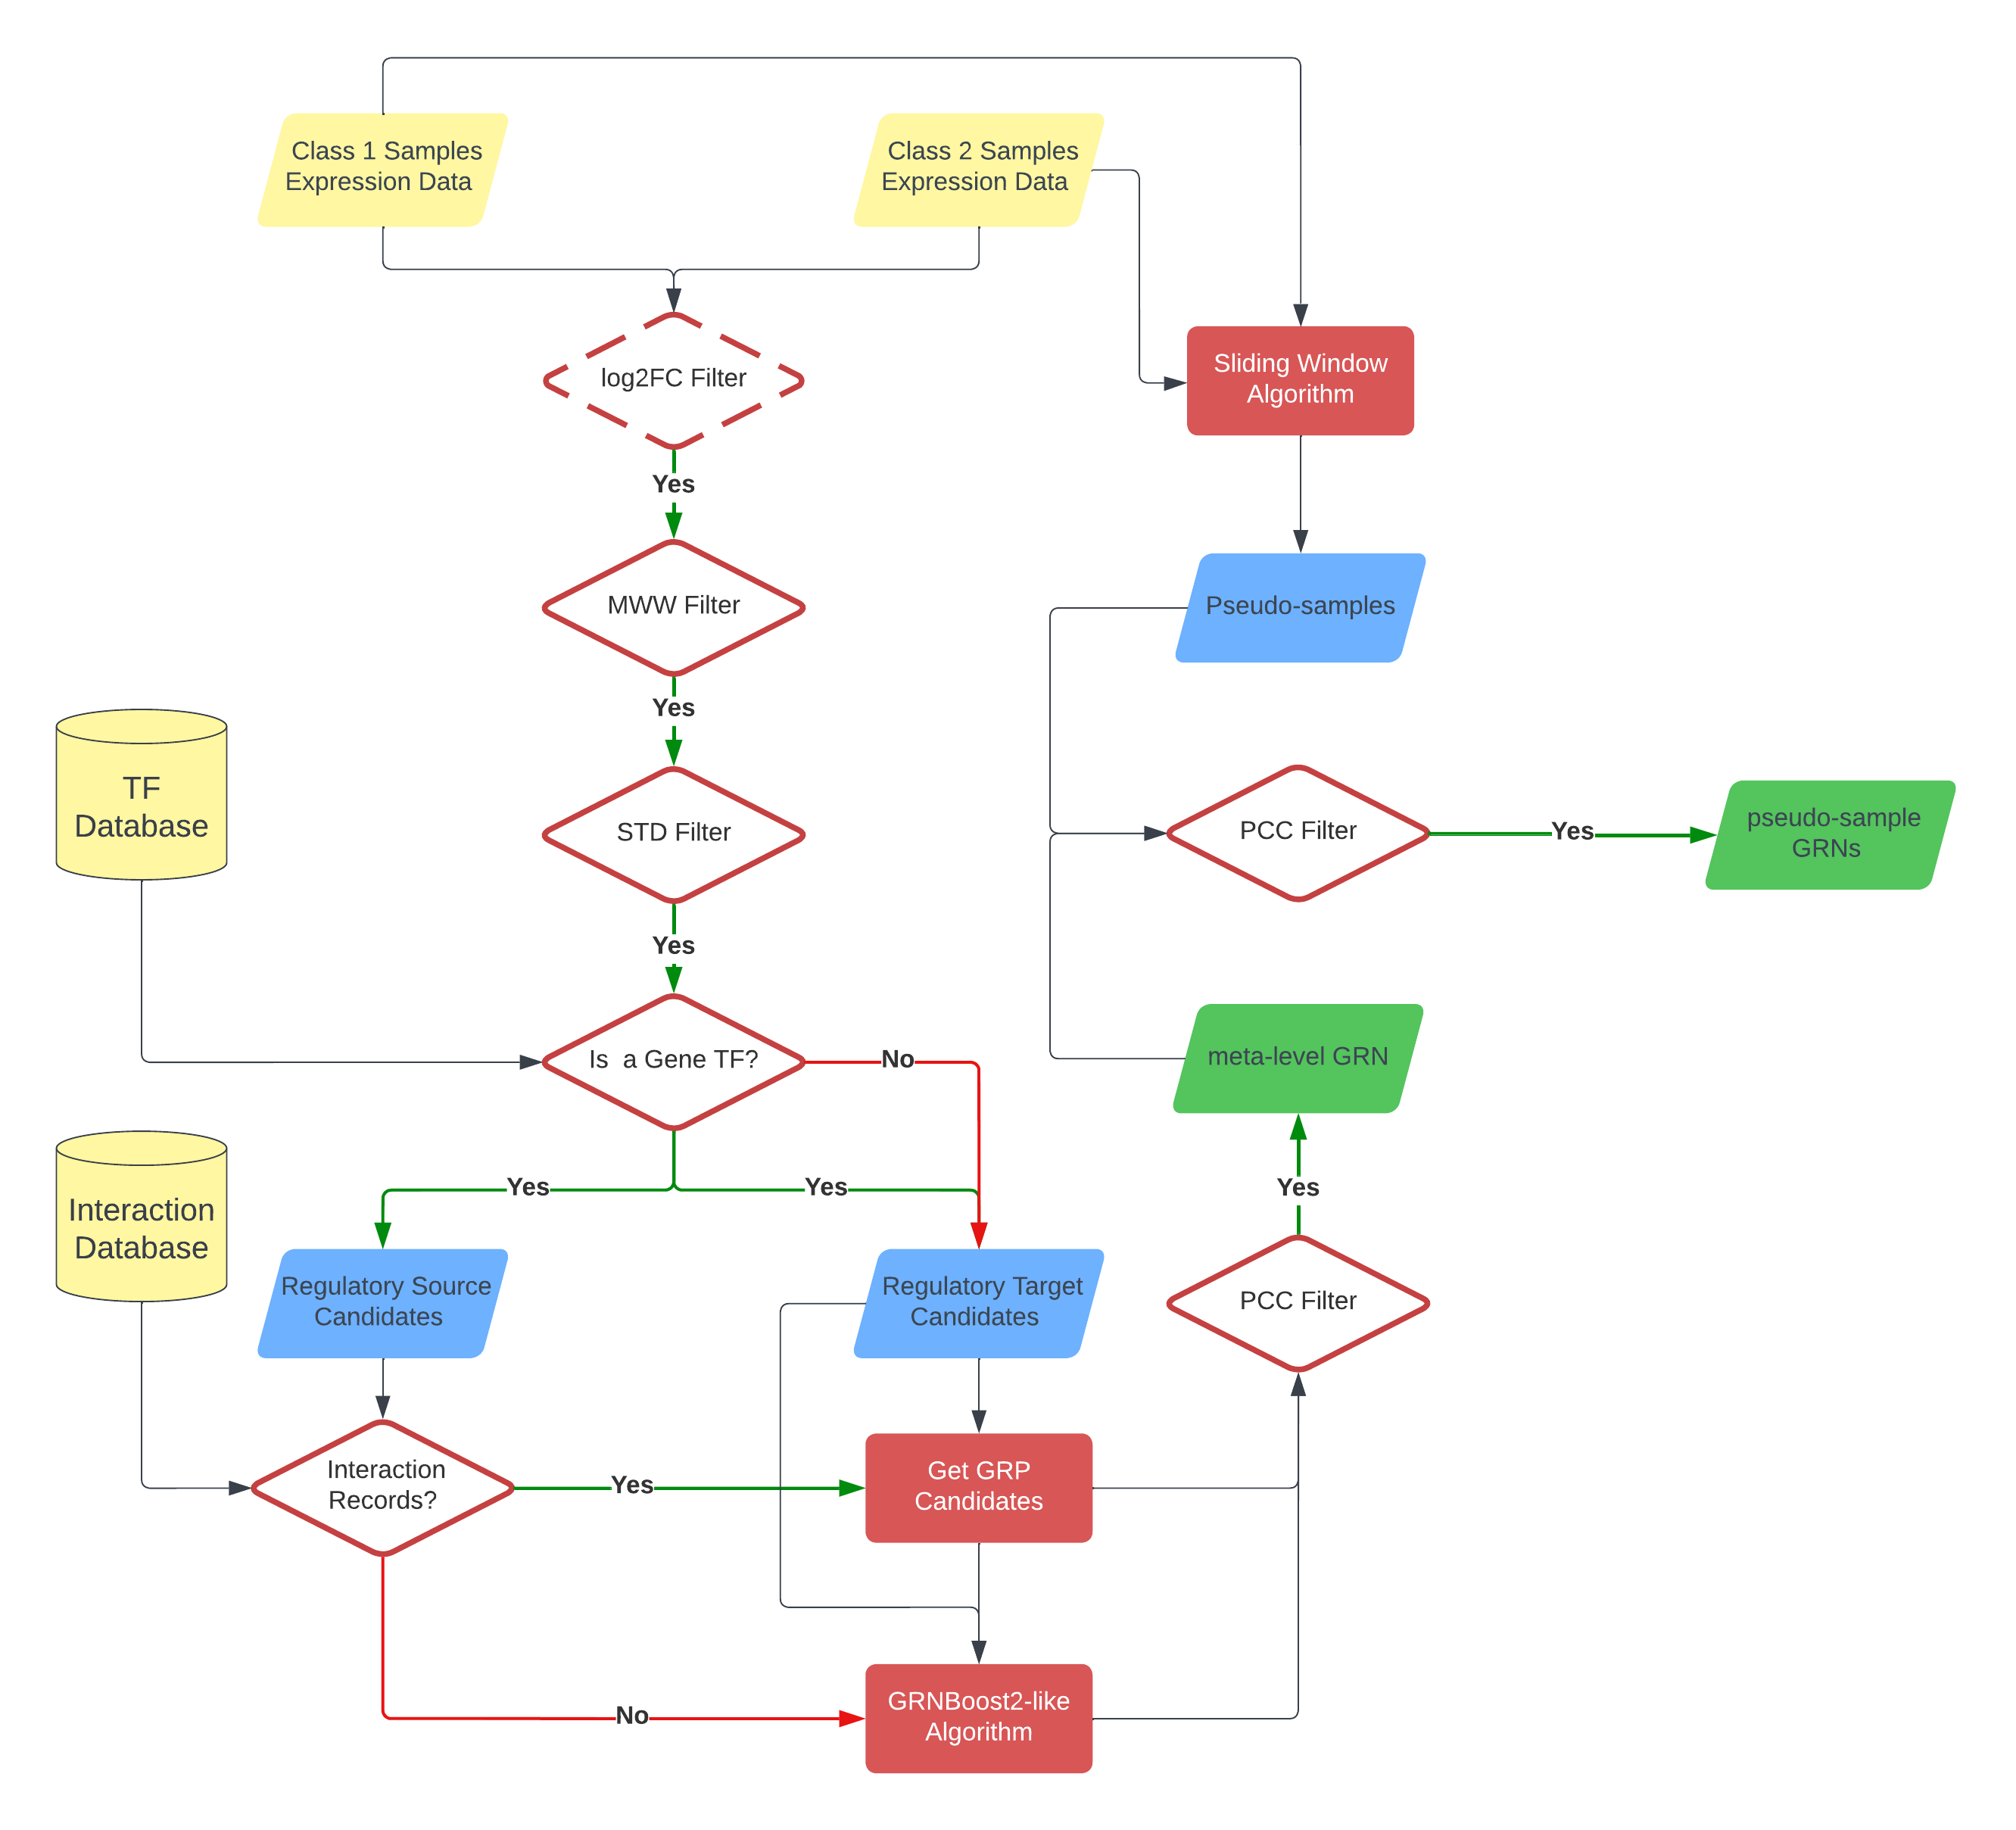
\includegraphics[width=0.8\linewidth, height=12cm, keepaspectratio,]{../images/data_preprocess_trans.png}
      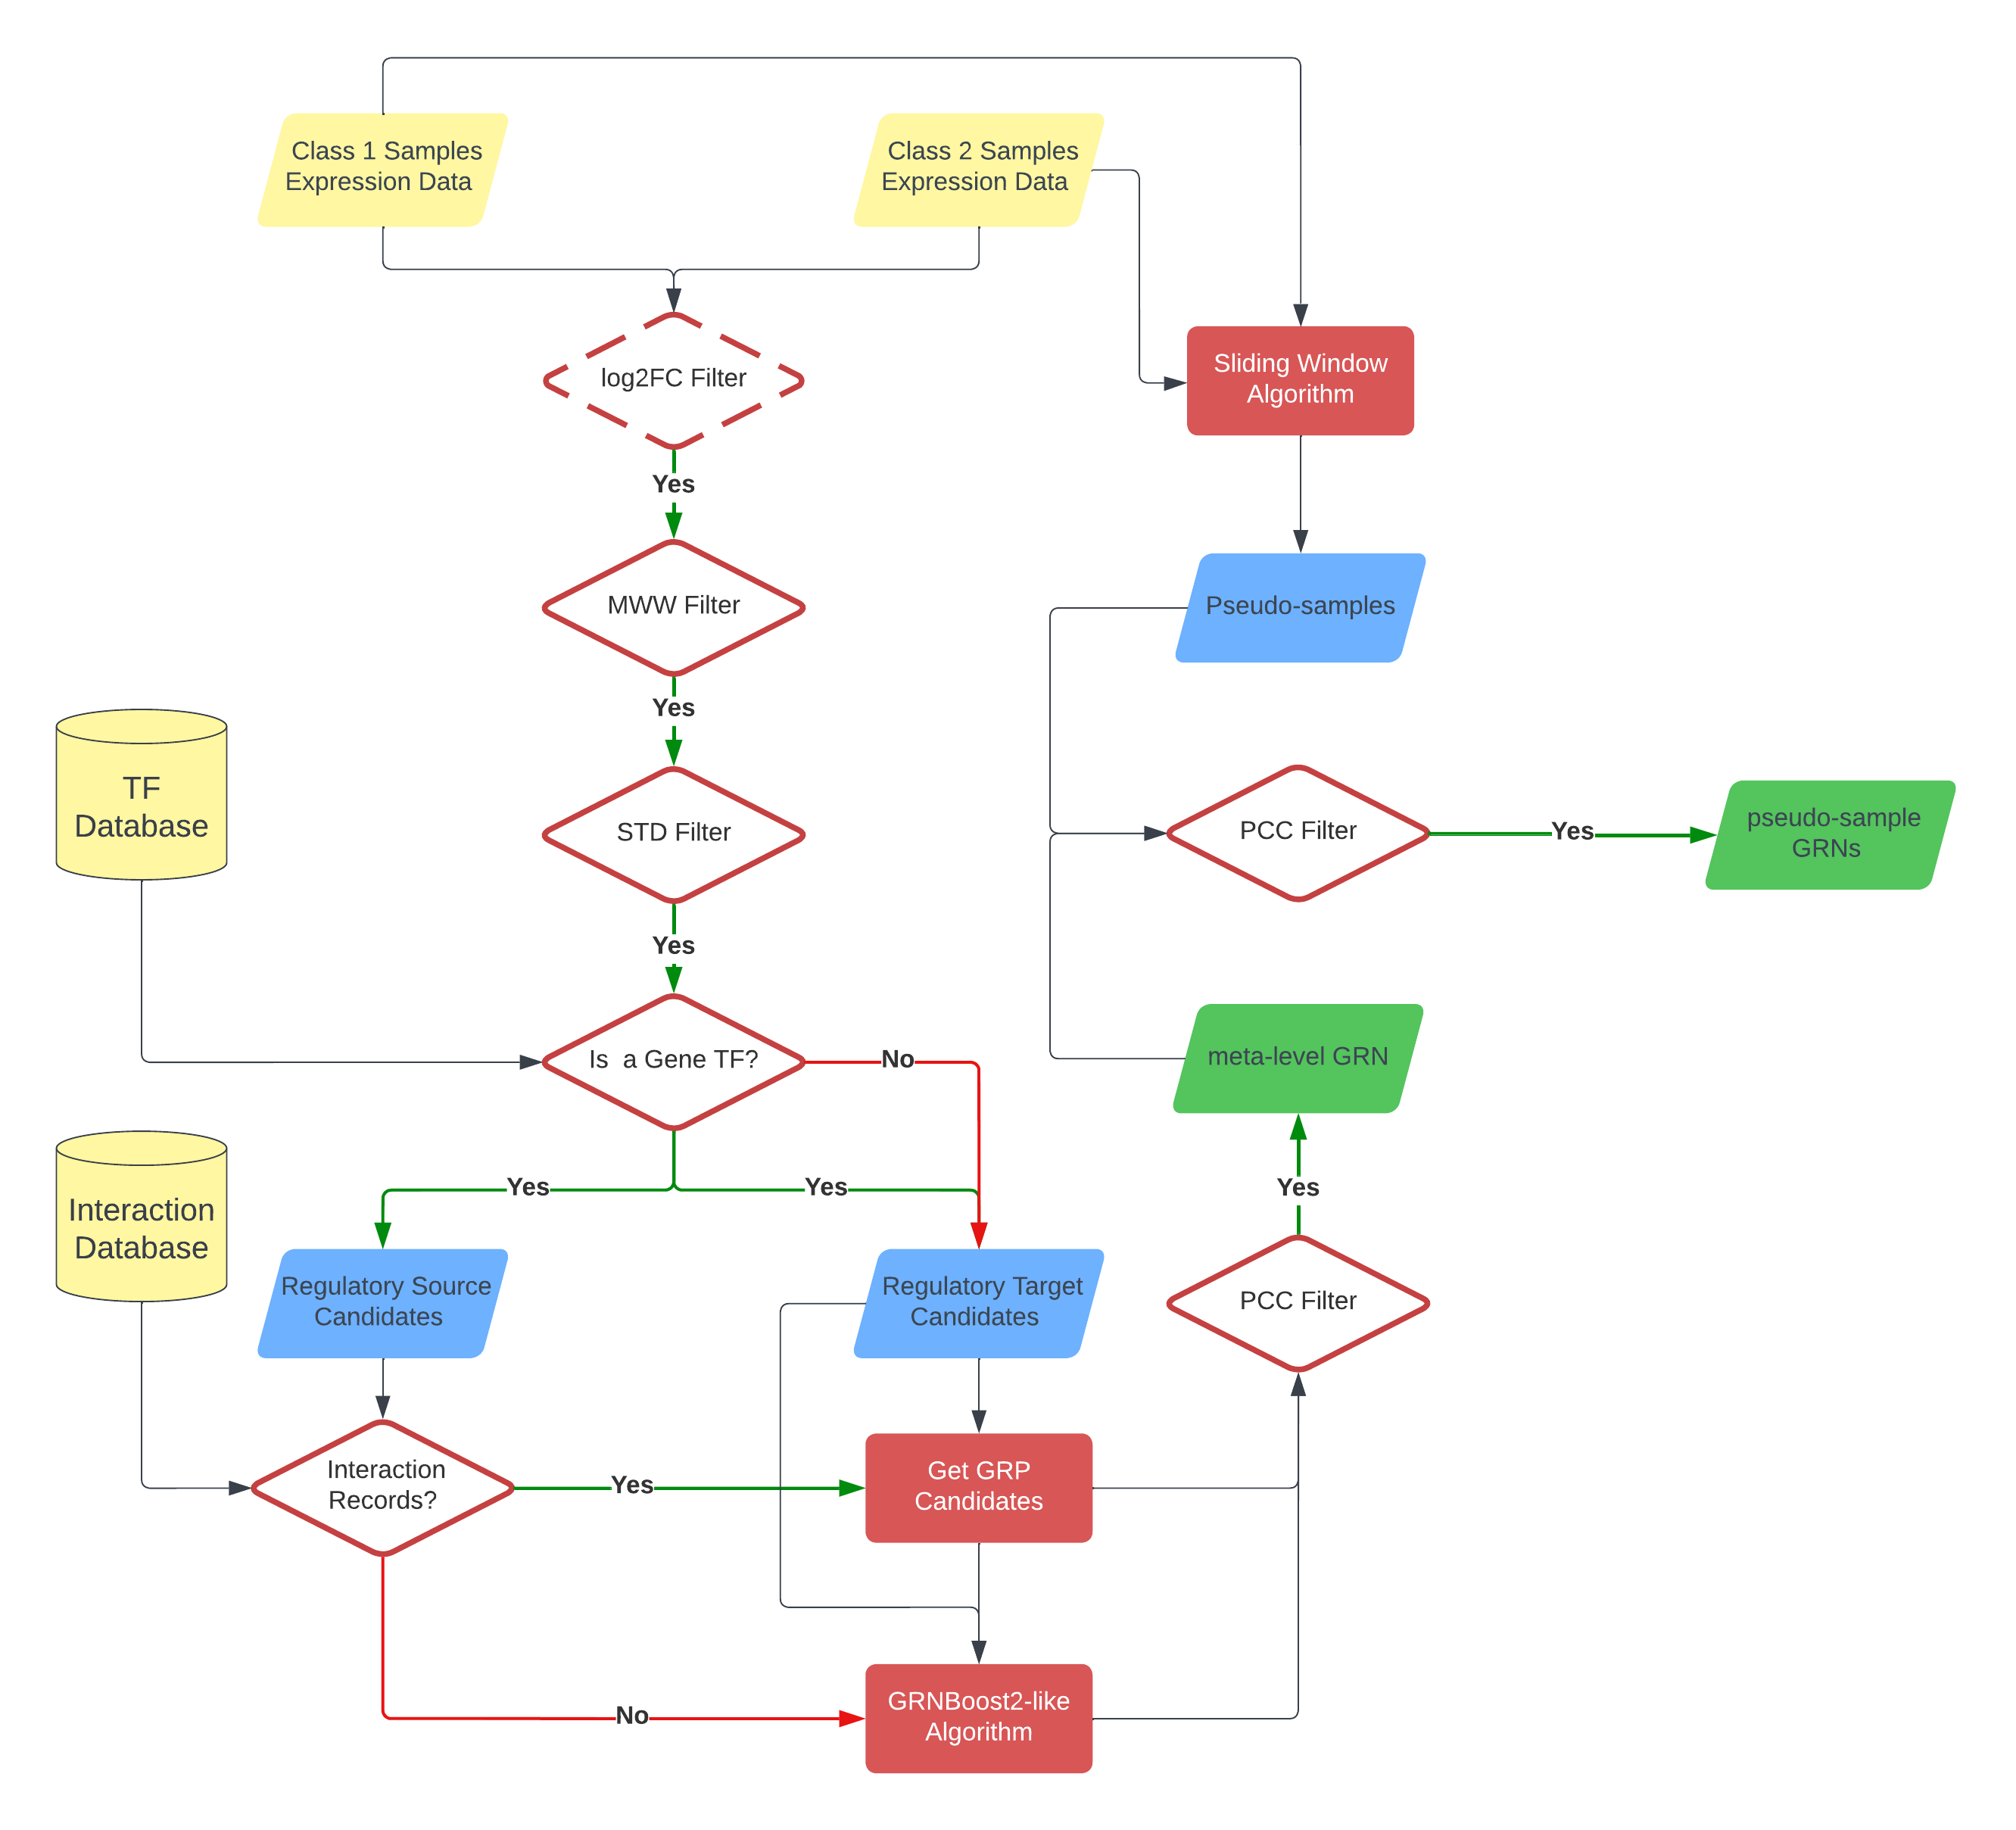
\includegraphics[width=0.8\linewidth, keepaspectratio,]{../images/data_preprocess_trans.png}
      \caption{
        Workflow to reconstruct meta-GRN and psGRNs.
        \textbf{\emph{(1)}} Filter genes from GEMs with log2FC filter(optional), MWW filter, and $\sigma$ filter.
        \textbf{\emph{(2)}} Find candidate GRP gene pairs from either interaction database or predictions made by \emph{GRNBoost2}\cite{grnboost2}-like algorithm.
        \textbf{\emph{(3)}} Filter candidate GRP gene pairs with PCC filter and reconstruct meta-GRN with validated GRPs.
        \textbf{\emph{(4)}} Generate pseudo-samples with SWA.
        \textbf{\emph{(5)}} Utilize GRPs in meta-GRN as generic guidance to form candidate GRPs for pseudo-samples.
        \textbf{\emph{(6)}} Filter every candidate GRP for all pseudo-samples with PCC filter and reconstruct psGRNs with validated GRPs.
      }
      \label{data_preprocess}
    \end{figure}

  \subsection*{Step 2: Classification model selection}
    \label{step2}
    Since AGEAS is not aiming to develop optimized model architectures for psGRN classification but gain insights from multiple models as divergent as possible, the main goal of this step is to select configurations of models capable to make correct psGRN classifications from provided configuration set.
    Regarding the fact that computational power is limited resource, portion of less efficient model configurations shall be pruned although interpreting success predictions of more classification models would lead to more comprehensive insight into sample class differences.
    Therefore, we apply a simple Hyperband\cite{hyperband}-based algorithm \ref{alg:one} which performs grid search for well-performing classification models with varying model training resource and pruning aggressiveness.


    %% This declares a command \Comment
    %% The argument will be surrounded by /* ... */
    \SetKwComment{Comment}{/* }{ */}
    \SetKwInput{kwInput}{Input}
    \SetKwInput{kwReturn}{Return}
    \RestyleAlgo{ruled}
    \begin{algorithm}
    \caption{Model selection algorithm}
    \label{alg:one}
    \kwInput{$R, C, I$ (default $I = 3$), $\alpha_{max}$(default $\alpha_{max} = 0.9$),  $k_{min}$(default $k_{min} = 0.5$)}
    $\alpha_{low} = \frac{1}{(2 ^ {I} - 1)}$\;
    % $X \gets x$\;
    \For{$i \in \{0, 1, ..., I-1\}$}{
      \eIf{$i == I-1$}{
        $\alpha = \alpha_{max}$\;
        % $X \gets X \times X$\;
        % $N \gets \frac{N}{2}$
        % \Comment*[r]{This is a comment}
      }{
        $alpha = 2^i \alpha_{low}$\;
      }
      $r = \alpha R$\;
      $P = \emptyset $\;
      \For{$c \in C$}{
        $p = run\_then\_evaluate(c, r, R)$\;
        Append $p$ to $P$\;
      }
      % \If{$N$ is odd}{
      %   }

      $k = max(1 - \alpha, k_{min}$)\;
  	  $C = top\_configs(C, P, k$)\;
    }
    \kwReturn{$C$}
    \end{algorithm}

    The model selection algorithm requires five inputs
    (1)$R$, the maximum amount of training resource, equivalent to all avaliable psGRNs
    (2)$C$, the total set of provided classification model configurations
    (3)$I$, the number of iterations for model pruning (default set as 3)
    (4)$\alpha_{max}$, the maximum portion of $R$ can be fed to single model (default set as 0.95)
    (5)$k_{min}$, the minimum portion of remaining model configurations will be kept by single pruning iteration (default set as 0.5).
    Furthermore, two functions are also required while need to be defined based on input model configurations:
    \begin{itemize}
    \setlength\itemsep{0em}
    \item \textbf{$run\_then\_evaluate(c, r, R)$}: trains classification model initialized using configuration $c$ for the allocated resource $r$, then returns prediction accuracy (ACC), the area under a receiver operating characteristic curve (AUROC)\cite{hanley_mcneil_1982} score, and total cross-entropy loss ($L_{CE}$) calculated through predicting sample class for all psGRNs $R$.

    \item \textbf{$top\_configs(C, P, k)$}: takes a set of model configurations $C$ with associated evaluation results $P$ and returns configurations having ACC, AUROC score, or $L_{CE}$ reaching top $k$ portion.
    \end{itemize}

    \noindent By default, AGEAS initializes with 128 model configurations utilizing 9 integrated classification algorithms listed in Table \ref{models}.

    \begin{table}[ht]
      \centering
      \begin{tabular}{|l|l|l|l|l|}
      \specialrule{.2em}{.1em}{.1em}
      \textbf{Algorithm} & \textbf{$\# \lambda$} & \textbf{Categorical} & \textbf{Continuous} & \textbf{$\#$ Configs}\\
      \specialrule{.2em}{.1em}{.1em}
      \multicolumn{5}{|l|}{\emph{Implemented with Pytorch}\cite{pytorch}} \\
      \hline
      Transformer & \textbf{14} & 4 & 10 & 32 \\
      \hline
      1D Convolutional Neural Network (1D-CNN) & \textbf{10} & 2 & 8 & 32 \\
      \hline
      Hybrid Convolutional Neural Network (Hybrid-CNN) & \textbf{10} & 2 & 8 & 32 \\
      \hline
      Gated Recurrent Unit (GRU) & \textbf{10} & 4 & 6 & 4 \\
      \hline
      Long Short-Term Memory (LSTM) & \textbf{11} & 4 & 7 & 4 \\
      \hline
      Standard Recurrent Neural Network (RNN) & \textbf{11} & 5 & 6 & 4 \\
      \specialrule{.2em}{.1em}{.1em}
      \multicolumn{5}{|l|}{\emph{Implemented with XGBoost}\cite{chen2016xgboost}} \\
      \hline
      Gradient Boosted Decision Trees (GBDT) & \textbf{18} & 5(1) & 13(4) & 16 \\
      \specialrule{.2em}{.1em}{.1em}
      \multicolumn{5}{|l|}{\emph{Implemented with scikit-learn}\cite{scikit-learn}} \\
      \hline
      Random Forests (RF) & \textbf{14} & 5(1) & 9(1) & 2 \\
      \hline
      Support Vector Machine (SVM) & \textbf{7} & 4 & 3(3) & 2 \\
      \specialrule{.2em}{.1em}{.1em}
      \end{tabular}
      \caption{
        \label{models}
        Classification model algorithms integrated in AGEAS with correspond numbers of hyperparameter and preset model configurations.
        Categorical hyperparameters and continuous numerical hyperparameters are clarifed beside total number of hyperparameters ($\# \lambda$).
        Conditional hyperparameters which are required for selected other hyperparameters are shown in brackets if there is any.
        $\#$ Configs indicates total amount of configurations AGEAS applies by default.
      }
    \end{table}

    The general architecture designs of 1D-CNN and Hybrid-CNN are implemented referring to 1D-CNN and 2D-Hybrid-CNN applied in recent cancer type prediction study.\cite{mostavi_chiu_huang_chen_2020}
    However, taking one convolution layer and adjacent max-pooling layer as a layer set, we implemented both CNN models with flexibilities on number of layer set, which is fixed as 1 in original research.
    An example of 1D-CNN with 2 convolution layer sets is illustrated in Figure \ref{1dCNN}.

    \begin{figure}[ht]
      \centering
      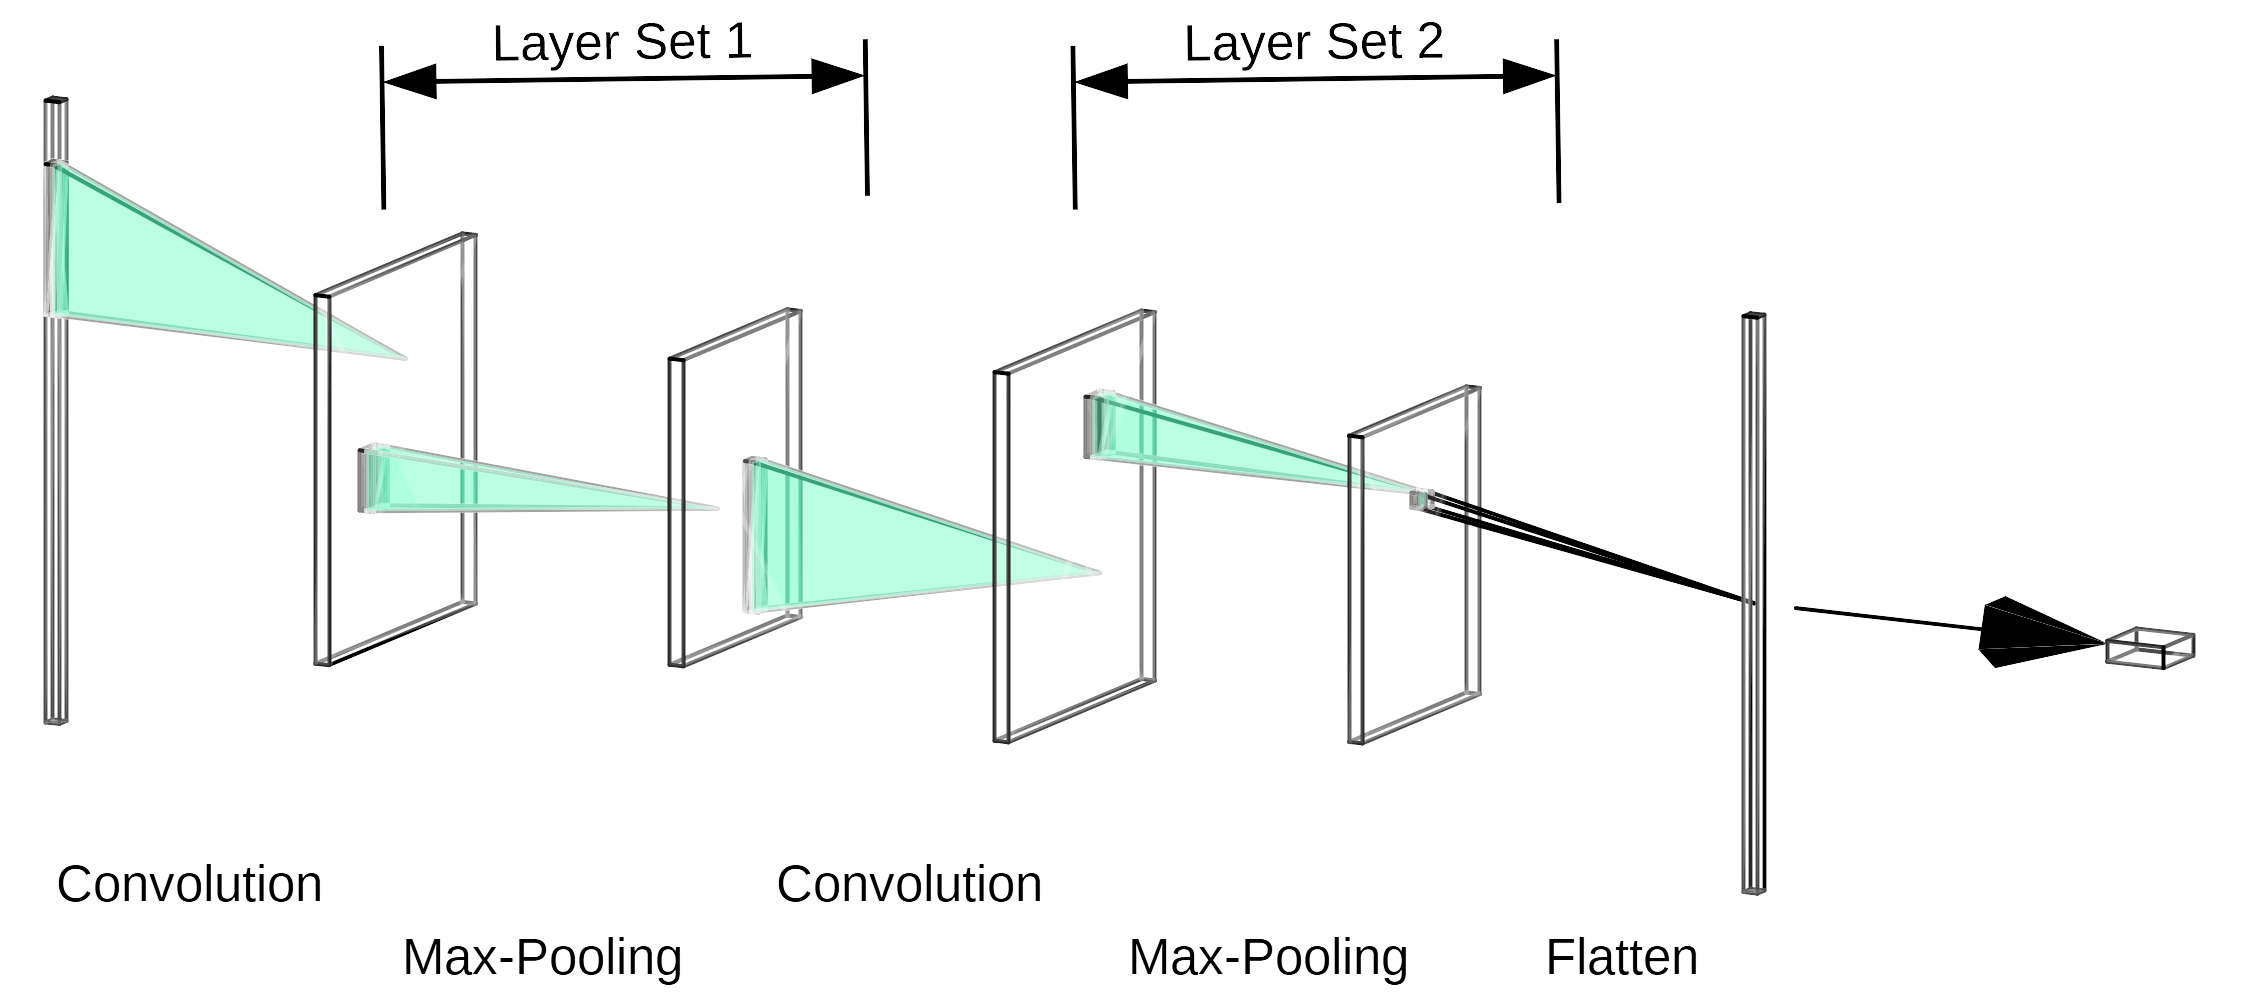
\includegraphics[width=0.8\linewidth]{../images/nn.png}
      \caption{1D-CNN with 2 convolution layer set.}
      \label{1dCNN}
    \end{figure}

    For transformer models, considering psGRNs are already be represented by numerical data matrix while GRPs should barely have positional relationships in the matrix, the embedding layer and positional encoding layer designed for input data tokenization in standard architecture \cite{transformer} are replaced with a single linear layer in AGEAS.

  \subsection*{Step 3: Feature selection}
    \label{step3}
    With selected well-performing models, AGEAS already can start repetition of model training and interpretation in \hyperref[step4]{Step 4} to extract key GRPs.
    However, few uninformative GRPs in training psGRNs merely relied by any model to make classification could be pruned in advance for saving computational power.
    Furthermore, to prevent classification models focusing on a small group of GRPs regardless of training psGRNs, GRPs draw excessive attention shall also be seperated from psGRNs to improve extraction comprehensiveness.
    Thus, in this step, AGEAS iteratively train classificaion models with dynamic $\alpha_{max}$ portion of psGRNs and obtain feature importance scores as described in \hyperref[features_importances]{subsection} below to find GRPs either scored extremely high or considerably low.

    More specifically, at each iteration, GRPs having z-scores ranked as bottom $b$ portion (default set as 0.1) are discarded.
    Also, an $i$-th ranked GRP will be seperated from psGRNs and passed to \hyperref[step5]{Step 5} directly if having z-score fulfilling the condition:

    \centerline{
      $Z_{score}^{i} \ge max(Z_{score}^{thread}, \frac{Z_{score}^{i-1}}{3}, 3 \cdot IQR)$
    }

    \noindent The $Z_{score}^{thread}$ is input z-score threshold (default set as 3.0), and $IQR$ stands for interquartile range calculated by the beginning of each iteration.\
    With this criterion, AGEAS ensures only GRPs draw significantly more attention shall be selected by each iteration despite the data distribution of varying z-score scalled importance values.

    By default, AGEAS iterates this feature selection step for 3 times.

    \subsubsection*{Feature importance estimation}
      \label{features_importances}
      AGEAS applies concept of The Shapley value\cite{roth_1988} for estimating importance of each input feature, equivalent to GRP of input psGRN, in any kind of classification model while making predictions.
      Specific Shapley value calculation or approximating methods are implemented with \emph{SHAP}\cite{lundberg2017unified} and applied to different algorithms as shown in Table \ref{shap}.
      Regarding the standard differences between feature importance estimating methods, we utilize \emph{softmax} function to normalize feature importances and define the normalized importance calculation function as:

      \centerline{$T(X) = softmax(\left\{ F(x) \right\}, x \in X)$}

      \noindent Here $X$ is total set of all features, and $F(x)$ is the importance estimating method of individual classification model being interpreted.\
      If the feature importances can be approached with internalized method $f(x)$, $F(x)$ is set as:

      \centerline{$F(x) = \frac{f(x)}{\sum_{x' \in X} f(x')}$}

      \noindent Otherwise, $F(x)$ is defined utilizing correctly classified input samples $S$, equivalent to psGRNs, with Shapley values $\phi$ of feature $x$ when predicting sample $s$ as class $c_1$ or class $c_2$:\

      \centerline{$F(x) = \sum_{s \in S}\frac{\left|\phi_{c_1,s}^{x}\right| + \left|\phi_{c_2,s}^{x}\right|}{2}$}

      \noindent After all selected classification models $M$ have been interpreted, we can intergrate the feature importances matrices weighted with corresponding models' $L_{CE}$ to one matrix $A$ as:\

      \centerline{
        $ A = \left\{ \sum_{m \in M}(1 - L_{CE}^{m})T_{m}(x) \right\}, x \in X $
      }

      \noindent Then, generalized importance values are obtained through z-score calculation and later sorted by descending order:\

      \centerline{
        $Z_{score} = \left\{\frac{a - \bar{A}}{\sigma_A}\right\}, a \in A$
      }

      \begin{table}[ht]
        \centering
        \begin{tabular}{|l|l|}
        \specialrule{.2em}{.1em}{.1em}
        \textbf{Algorithm} & \textbf{SHAP\cite{lundberg2017unified} Method}\\
        \hline
        Transformer & Gradient Explainer \\
        \hline
        1D-CNN & Deep Explainer \\
        \hline
        Hybrid-CNN & Deep Explainer \\
        \hline
        GRU & Gradient Explainer \\
        \hline
        LSTM & Gradient Explainer \\
        \hline
        RNN & Gradient Explainer \\
        \hline
        GBDT\textbf{*} & Tree Explainer \\
        \hline
        RF & Tree Explainer \\
        \hline
        SVM\textbf{*} & Linear Explainer / Kernel Explainer\\
        \specialrule{.2em}{.1em}{.1em}
        \end{tabular}
        \caption{
          \label{shap}
          Classifier algorithms with applicable Shapley value approximating methods.
          Algorithms marked with \textbf{*} have internalized feature importance estimating methods which will be applied with higher priority than Shapley value based methods.
          GBDT implemented with \emph{XGBoost}\cite{chen2016xgboost} can have feature importance approximated with average weight gain at each split involving the feature.
          Linear SVM implemented with \emph{scikit-learn}\cite{scikit-learn} can have the importance estimated with feature coefficient or using Linear Explainer.
          However, for SVM with kernel function, the feature coefficient estimation would be inappropriate, and feature importances should be approximated with Kernel Explainer.
        }
      \end{table}

  \subsection*{Step 4: Top GRP extraction}
    \label{step4}
    To extract GRPs can effectively define sample class differences, AGEAS iteratively initializes classification models with configurations gained from \hyperref[step2]{Step 2}, trains them with randomly selected $\alpha_{max}$ portion of psGRNs scaled after \hyperref[step3]{Step 3}, and interpret every models' correct predictions as mentioned in \hyperref[features_importances]{subsection} above.
    At each iteration, AGEAS receives a z-score scaled feature importance matrix $A$ and add up each GRP's score accordingly from matrix $A'$ kept from previous iteration if there is one.
    Then, top $a$ (default set as 100) ranked GRPs having z-score greater than $0.0$ extracted from $A$ are compared with GRPs extracted from $A'$ by same setting.
    If less than $d$ (default set as 0.05) portion of GRPs are distinct for GRP sets stratified from $A$ and $A'$, AGEAS will consider the GRP extration result from this iteration being consistent with previous one.
    Extraction iteration will terminate if either encountering $n$ (default set as 3) continuous consistent result or running out of preset iteration number (default set as 10).
    All feature importance scores in matrix $A$ from last iteration are divided by total extraction iteration number processed, and top $a$ ranked GRPs are considered as key GRPs for sample class differentiation and passed to next step.

  \subsection*{Step 5: Key network reconstruction}
    \label{step5}
    Analoging every GRP previously extracted or seperated with high z-score in \hyperref[step3]{Step 3} as a directional edge connecting two gene vertices, equivalent to a TF and a gene, in graph theory, AGEAS attempts to reconstruct a network graph representing regulatory differences between query sample classes.
    Since there is no guarantee on all GRP edges can be connected, some regulatory relationships between gene vertices could be missed.
    Hence, AGEAS utilizes meta-GRN gained from \hyperref[step1]{Step 1} to find GRPs which can further elucidate the regulatory relationships and adds the GRPs back to the network graph.

    For a limited iteration time (default set as  1), AGEAS exhaustively search meta-GRN for TFs which can directly regulate any genes or TFs already covered in the network graph and add the returned TFs as new vertices.
    Next, any GRP in meta-GRN capable to connect two distinct vertices will be added if it is not covered yet.
    The network graph after expansion above represents the key genetic regulatory differences AGEAS extracted from input sample classes.


\section*{Results}
  \label{res}
  To assess AGEAS's predictive power, we first applied AGEAS to study somatic reprogramming to induced pluripotent stem cells (iPSC) achieved in mice by the year 2006, \cite{yamanaka_2006} milestone discovery of cell plasticity. \cite{cell_repro_review}
  With $\sigma$ thread set to 2.0 for constraining total GRP amount in psGRNs, public scRNA-Seq based gene expression matrices (GEMs) of embryonic stem cells (ESCs) and mouse embryonic fibroblasts (MEFs) shown in Table \ref{geo_table} were used as input.
  The extraction result can be summarized as TF regulons, collections of a TF and corresponding direct regulatory targets, and TFs forming largest regulons with extracted GRPs are shown in Figure \ref{result_figs}(a).
  Among TFs with sizeable regulons, Pou5f1 (Oct4), Nanog, and Sox2 are also most differentially expressed in MEF and ESC samples.
  Thus, we can infer these TFs as import factors closely related with cell type differences.
  Multiple previous studies confirmed that all of Oct4, Nanog, and Sox2 are playing important role in maintaing pluripotency \cite{niwa_2007} and inducing conversion from somatic cell to iPSC. \cite{yamanaka_2006, ips7f, ipsOK, oct4_nanog_sox2_lin28, oct4_nanog_sox2}

  To further address AGEAS's applicability and limitation, we applied AGEAS to three other scRNA-Seq based studies in distinct research areas.
  With all default settings and analytical procedure applied above, we can assess AGEAS's performance in following scenarios with public data set shown in Table \ref{geo_table}:

  \begin{itemize}
    \setlength\itemsep{0em}
    \item {\textbf{Dopaminergic neuron generation}}:

      Analyzing difference between human iPSC-derived radial glial / neuronal co-culture, as neural progenitors,\cite{ASCL1_dopaminergic_neuron_2021} and tyrosine hydroxylase (TH) expressing purified dopaminergic (DA) neurons, we address the applicability of AGEAS on cell subtype differentiation problems.

      From extracted TFs shown in Figure \ref{result_figs}(b), we hypothesize ISL1, PHOX2B, and ELF3, referring to their correspond regulon sizes and differential expression profiles, are regulating essential functions differentiating DA neurons from neural progenitors.
      Both ISL1 and PHOX2B were found related with DA phenotype in previous studies:
      ISL1 is essential for differentiation of prethalamic DA neurons,\cite{isl1_da}
      and PHOX2B is connected with TH expression influencing DA neuron development and improving DA activity. \cite{phox2_caudal_da, phox2_rat_da}
      Moreover, ELF3 was found to be neuronal precursor cell marker associated with neural stem cell development, \cite{ELF3_precursor_marker} consistent with it's high expression level in neuronal co-culture class.

      EBF1, which forms the largest regulon with extracted GRPs, was determined as key neuronal differentiation regulator in the ventral telencephalon, nature source of neuronal and glial cells. \cite{ebf1_striatum, ebf1_cell_diff}
      Furthermore, EBF1 plays important role in mesodiencephalic DA neuron migration. \cite{ebf1_migration}
      ASCL1, found as necessary factor regulating DA neurotransmitter selection by original research where we retrieved scRNA-Seq data,\cite{ASCL1_dopaminergic_neuron_2021} is also forming substantial regulon.
      % SOX2 and NR3C1 also have reports in neuronal differentiation...
      Remarkably, within extracted network, ASCL1 appears to act as upstream regulator of several large TF regulons, including ISL1 and PHOX2B, in purified DA neurons.

    \item {\textbf{Postnatal cardiomyocyte maturation}}:

      To address the performance of AGEAS while analyzing cell physiological development, scRNA-Seq data of cardiomyocytes (CMs) in postnatal day 7 mice (P7) and day 28 mice (P28) are used as input for extracting key genetic regulatory elements in postnatal cardiomyocyte maturation.

      Following same regulon size and expression profile based analytical procedure, we primarily investigated three TFs shown in Figure \ref{result_figs}(c): Sp1, Esr1 ($ER\alpha$), and Cebpb.
      Previous studies demonstrated that Sp1 promotes CM hypertrophy \cite{sp1_hypertrophy} and maturation of electrophysiology and $Ca^{2+}$ handling. \cite{Sp1_electrophysiologt, CM_mature}
      % trans-activation of the SERCA2 promoter
      Esr1 was found modulating myocardial development for postnatal cardiac growth,\cite{esr1_cm, esr1_cm_growth} and Cebpb's role as repressor of CM growth and proliferation while preventing pathological CM hypertrophy also demonstrated by several studeis.\cite{cebpb_1, cebpb_2}

      Other TFs known playing important roles in CM maturation, such as Srf, \cite{CM_mature, cebpb_1} Nkx2-5,\cite{cebpb_1, nkx25, CM_posnatal_mature} and Yap1,\cite{CM_mature, yap1, CM_posnatal_mature} are also forming sizeable regulons in GRN atlas returned by AGEAS.

    \item {\textbf{Hepatic stellate cell activation in $CCl_4$ induced liver fibrosis}}:

      Here we address AGEAS's applicability on cell pathological development studies through analyzing hepatic stellate cells (HSCs) in mice liver administrated with chronic carbon tetrachloride ($CCl_4$) for 6 weeks and according portal fibroblasts (PF) simulating activated HSCs.

      Within TFs shown in Figure \ref{result_figs}(d), we suppose Lhx2, Osr1, and Ebf1 are regulating HSC activation considering their correspond TF regulon sizes and expression changes.
      Previously, Lhx2 was found indispensable for quiescent HSCs. \cite{lhx2_fibro, Lhx2_hsc_1}
      Extensive studies found Osr1 related with pathological fibrogenic process in liver fibroblast. \cite{osr1_1, osr1_2, osr1_3}
      However, little literature address Ebf1's role in liver fibrosis.
      One recent study reported the expression of Ebf1 increases concurrent with Acta2, marker gene of myofibroblast formation\cite{acta2_myofb_marker} which is essential for fibrosis, in wound fibroblast. \cite{ebf1_fibroblast}
      Also, Ebf1 was found associated with lung fibrosis.\cite{ebf1_lung}

      Furthermore, Mef2c, forming largest TF regulon, has been well-documented as key regulator in HSC activation. \cite{mef2c_1, mef2c_2, mef2c_3}

  \end{itemize}

  \begin{figure}
    \begin{subfigure}{0.49\linewidth}
      \centering
      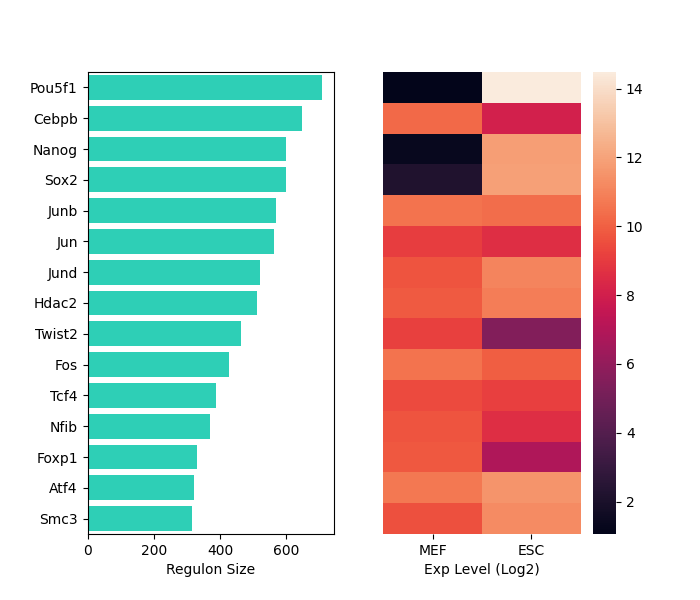
\includegraphics[width=\linewidth, keepaspectratio,]{../images/MEF_ESC_top.png}
      \caption{}
    \end{subfigure}
    \begin{subfigure}{0.49\linewidth}
      \centering
      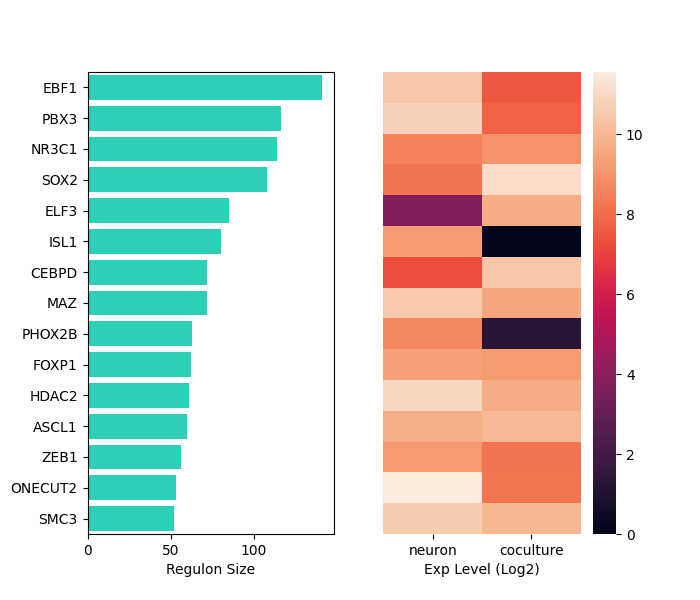
\includegraphics[width=\linewidth, keepaspectratio,]{../images/N_cocul_top.png}
      \caption{}
    \end{subfigure}

    \begin{subfigure}{0.49\linewidth}
      \centering
      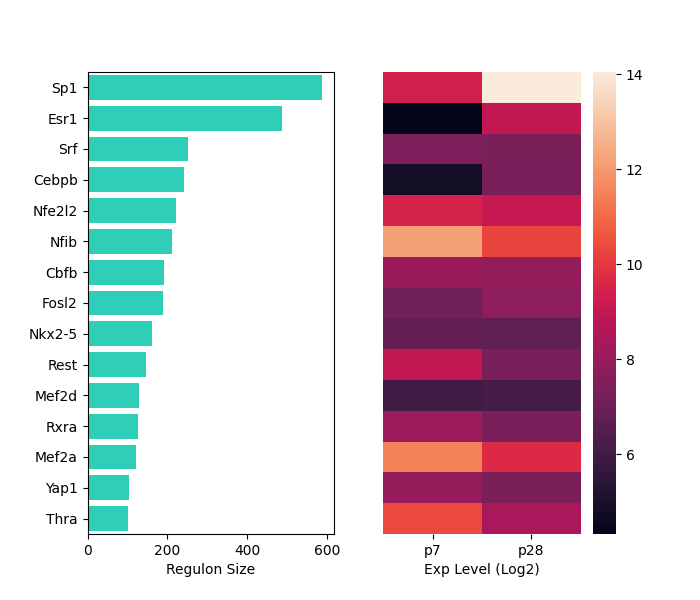
\includegraphics[width=\linewidth, keepaspectratio,]{../images/CMp7d_CMp28d_top.png}
      \caption{}
    \end{subfigure}
    \begin{subfigure}{0.49\linewidth}
      \centering
      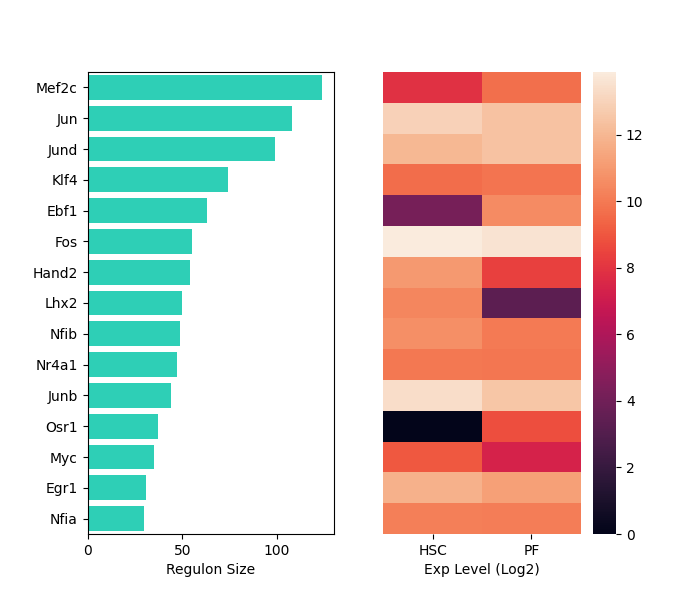
\includegraphics[width=\linewidth, keepaspectratio,]{../images/HSCp6w_PFp6w_top.png}
      \caption{}
    \end{subfigure}

    \caption{
      TFs forming largest regulons with GRPs extracted by AGEAS.
      Each TF has regulon size indicating amount of direct regulatory genes and $log_2$ gene expression levels in binary sample classes.
      \textbf{\emph{(a)}} Mouse embryonic fibroblast vs. Embryonic stem cell
      \textbf{\emph{(b)}} Purified dopaminergic neuron vs. Radial glial/neuronal co-culture
      \textbf{\emph{(c)}} 7 days postnatal cardiomyocyte vs. 28 days postnatal cardiomyocyte
      \textbf{\emph{(d)}} Hepatic stellate cell vs. Portal fibroblast (both after 6 weeks of CCl4 administration)
    }
    \label{result_figs}
  \end{figure}

  To demonstrate empirically the predictive capabilities...
  Since Lhx2's expression pattern is strongly favoring HSC than PF, and previous study proved Lhx2 KO promotes liver fibrosis\cite{lhx2_fibro}...
  We suppose overexpression of Lhx2 could halt HSC as quiescent in order to prevent pathological fibrogenic process...
  In vitro experiment goes here...

  % \begin{table}[ht]
  %     \centering
  %     \begin{tabular}{|l|l|l|l|}
  %       \hline
  %       \textbf{Gene} & \textbf{Main Exp Class} & \textbf{$|log2FC|$} & \textbf{Description}  \\
  %       \hline
  %       Mef2c & 1 & 1.82 & sth \\
  %       \hline
  %     \end{tabular}
  %     \caption{
  %       \label{ccl4liver_result}
  %       In total of 35 Genes
  %     }
  % \end{table}

\section*{Discussion}
  \label{disc}

  In present study, we showed AGEAS's applicability in analyzing scRNA-Seq derived data in cell reprogramming development, cell subtype differentiation .
  According to test cases so far, key TFs closely related with sample class difference appear to either form substantial regulon with extracted GRPs or high regulatory influence on other key genes.
  Without any previous knowledge on studying CSs, Gene Ontology (GO) enrichment analysis can potentially narrow down key cellular functions changed in different CSs.

  However, larger scales of applicability test can further confirm AGEAS's capability on guiding frontier researches.
  While more computational resources become available, other classification algorithms and according interpretation methods will be added and tested with current version on larger scales.


  With result achieved so far, we anticipate that AGEAS will become useful in providing insightful advices on not only learning differences between CSs and cell subtypes, but also finding key GFs to induce CS conversions unachievable so far.

  Limitations...
  Fidelity of GRPs...
  Reconstruct GRN with ATAC-Seq by motif enrichment instead of ChIP-Seq... (especially considering technology like Share-Seq which can perform scRNA-Seq with scATAC-Seq in same cell simultaneously...)
  Apply AGEAS on tissue studies with spatial transcriptomics...



% \section*{Conclusion}
  % \label{conc}
  % Conclusion goes here

\bibliography{reference}

% For data citations of datasets uploaded to e.g. \emph{figshare}, please use the \verb|howpublished| option in the bib entry to specify the platform and the link, as in the \verb|Hao:gidmaps:2014| example in the sample bibliography file.

\section*{Author contributions statement}
\textbf{J.Y.}: Methodology, Software, Writing- Original draft preparation, Project administration
\textbf{M.N.}: Methodology, Software
\textbf{J.T.}: Writing - Review \& Editing, Project administration

\section*{Additional information}
All scRNA-Seq datasets are retrieved from Gene Expression Omnibus(GEO) as described in the Table below.

\begin{table}[ht]
  \centering
  \begin{tabular}{|l|l|}
  \specialrule{.2em}{.1em}{.1em}
  \textbf{Sample Class} & \textbf{Accession number}\\

  \specialrule{.2em}{.1em}{.1em}
  \multicolumn{2}{|l|}{GSE103221} \\
  \hline
  MEF & GSM3629847 \\
  \hline
  ESC & GSM3629848 \\

  \specialrule{.2em}{.1em}{.1em}
  \multicolumn{2}{|l|}{GSE137720 } \\
  \hline
  $CCl_4$ a6w hsc & GSM4085625 \\
  \hline
  $CCl_4$ a6w pf & GSM4085627 \\
  % \hline
  % healthy hsc & GSM4085623 \\
  % \hline
  % healthy pf & GSM4085626 \\

  \specialrule{.2em}{.1em}{.1em}
  \multicolumn{2}{|l|}{GSE185275 } \\
  \hline
  glial/neuronal co-culture & GSM5609927 \\
  \hline
  purified DA neurons & GSM5609930 \\

  \specialrule{.2em}{.1em}{.1em}
  \multicolumn{2}{|l|}{GSE156482 } \\
  % \hline
  % p4 cm & GSM4732219 \\
  \hline
  p7 CM & GSM4732221 \\
  \hline
  p28 CM & GSM4732225 \\
  % \hline
  % p28 ncm & GSM4732226 \\

  \specialrule{.2em}{.1em}{.1em}
  \end{tabular}
  \caption{
    \label{geo_table}
  }
\end{table}

% $CASH$        & Combined Algorithm Selection and Hyperparameter optimization\\
\end{document}
